\documentclass[onecolumn, 11pt, draftclsnofoot]{IEEEtran}

\usepackage{epsfig,graphics,epsf,amsfonts,color,mathrsfs,amssymb,bm,caption,algorithm,algorithmic}
\usepackage{url}

\usepackage{amsmath}
\newcommand{\bsb}{\boldsymbol}
\newcommand{\mb}{\mathbf}
\newcommand{\mc}{\mathcal}
\newcommand{\mexpc}{\mathrm{E}}
\newcommand{\ve}{\mathrm{vec}}
\newcommand{\toep}{\mathcal{T}}
\newcommand{\tr}{\mathrm{tr}}
\newcommand{\tred}{\color{red}}
\textheight=9.2in
\DeclareCaptionLabelFormat{lc}{\MakeLowercase{#1}~#2}
\captionsetup{labelfont=sc,labelformat=lc}
\renewcommand{\figurename}{Figure}
\renewcommand{\theequation}{R\arabic{equation}}

\usepackage[numbers]{natbib}

%\hyphenation{op-tical net-works semi-conduc-tor}
\begin{document}
The authors appreciate the helpful comments and suggestions from both reviewers. 
Throughout this response letter, we will follow the following notational
rules for citations and references:
\begin{itemize}
  \item Citations: references in this response letter are cited with prefix
  ``R'' (e.g. [R 1]) whereas references in the original manuscript are cited
  without prefix (e.g. [1]).
  \item Equations: equations in this response letter are referred to as
  ``Eq.~(R1)''  while those in the original manuscript as ``Eq.~(1)''.
  \item Figures: figures in this response letter are referred to as
  ``FIGURE~1''  while those in the original manuscript as ``Fig.~1''.
\end{itemize}

\begin{center}
  {\LARGE \textbf{Authors' Response to Reviewer 1}}
\end{center}

% ~\citep[R][]{cheng2013thermal}
% \begin{align}
%   sfsdf
%   \label{eq:test}
% \end{align}
% \eqref{eq:test}
% \begin{figure}[!t]
%   \centering
%   \includegraphics[width=0.75\columnwidth]{./figs/test.eps}
%   \caption{Average throughput.}
%   \label{fig:test}
% \end{figure}
% Fig.~\ref{fig:test}

%%%%%%%%%%%%%%%%%%%%%%%%%%%%%%%%%%%%%%%%%%%%%%%%%%%%%%%%%%%%%%%%
\noindent
\emph{1. The signal model needs further work: $p$ is reported as “index” before
(1) and something to be demodulated in (3); in (1), which is the transmit
vector/symbol? }

\noindent \textbf{Authors' response:}
Thank you for the comment. As mentioned in the first paragraph in Section
II, the transmitted vector corresponding to two symbols are
$\bm{\phi}^(m)[p] = [\psi_1^{(m)}[p], \psi_2^{(m)}[p]]^T$, where
$p=0,\ldots,Q-1$ is the index/label corresponding to a bit sequence of length
$\log_2Q$, and in Eq.~(1) the transmitted symbols at the two RRHs are
$\psi_1^{(m)}[p]$ and $\psi_2^{(m)}[p]$, respectively. For instance, for 16-QAM where $Q=16$, in
one round of (re)transmission every 4 bits can be mapped to 2 constellation
symbols as in TABLE~\ref{table:mapping} and FIGURE~\ref{fig:mapping}.

To demodulate the information bits is equivalent to figuring out label $p$ from
the received signal $\mathbf{y}^{n}$ where $n=0,\ldots,m$ denote different
rounds of (re)transmissions. Since the noise is Gaussian distributed and we
assume perfect CSI at the receiver, the maximum-likelihood rule is in the form
of Eq.~(3).

To prevent possible confusion from our readers, we rephrase the description of
our signal model in the first paragraph of Section II, using similar
terminology as [4]. Most notebaly, we have renamed $p$ as ``label'' instead of
``index'' throughout the manuscript.

\begin{table}[!t]
  \renewcommand{\arraystretch}{1.3}
  \caption{Mapping from bits to constellation symbols.}
  \label{table:mapping}
  \centering
  \begin{tabular}{c|c|c|c}
    \hline
     bits & $p$ & $\psi_1^{(m)}[p]$ & $\psi_2^{(m)}[p]$  \\
    \hline
    0000 & 0 & $-3+3j$ & $-1+1j$ \\
    0001 & 1 & $-3+1j$ & $-1-3j$ \\
    0010 & 2 & $-3-3j$ & $-1-1j$ \\
    0011 & 3 & $-3-1j$ & $-1+3j$ \\
    0100 & 4 & $-1+3j$ & $+3+1j$ \\
    0101 & 5 & $-1+1j$ & $+3-3j$ \\
    0110 & 6 & $-1-3j$ & $+3-1j$ \\
    0111 & 7 & $-1-1j$ & $+3+3j$ \\
    1000 & 8 & $+3+3j$ & $+1+1j$ \\
    1001 & 9 & $+3+1j$ & $+1-3j$ \\
    1010 & 10 & $+3-3j$ & $+1-1j$ \\
    1011 & 11 & $+3-1j$ & $+1+3j$ \\
    1100 & 12 & $+1+3j$ & $-3+1j$ \\
    1101 & 13 & $+1+1j$ & $-3-3j$ \\
    1110 & 14 & $+1-3j$ & $-3-1j$ \\
    1111 & 15 & $+1-1j$ & $-3+3j$ \\
    \hline
  \end{tabular}
\end{table}

\begin{figure}[htb]
  \begin{minipage}[b]{0.48\linewidth}
    \centering
    \centerline{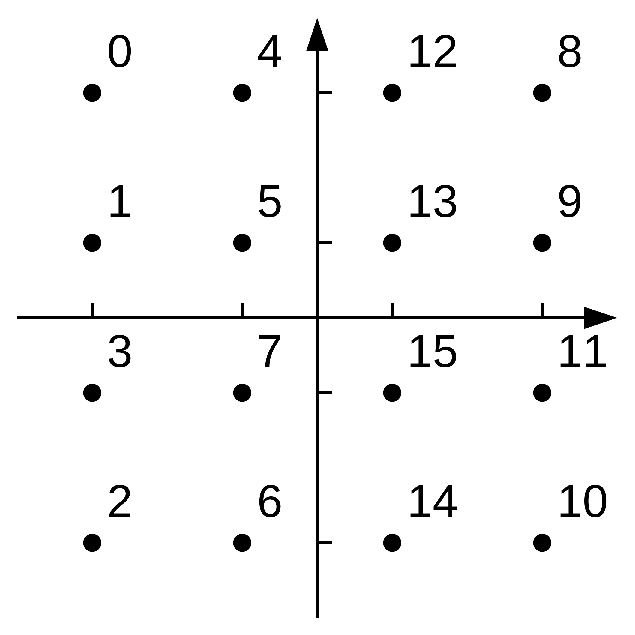
\includegraphics[width=4.0cm]{./figs/gray.eps}}
    \centerline{(a) $\psi_1^{(m)}[p]$ (Gray mapping)}\medskip
  \end{minipage}
  \hfill
  \begin{minipage}[b]{.48\linewidth}
    \centering
    \centerline{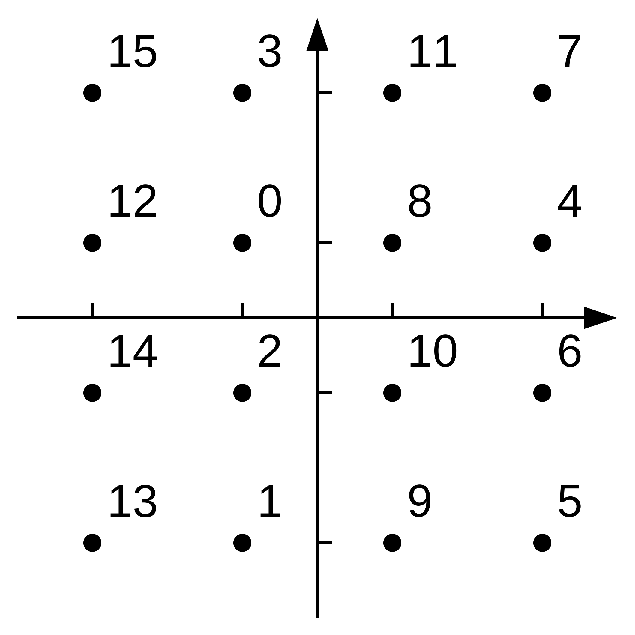
\includegraphics[width=4.0cm]{./figs/karim.eps}}
    \centerline{(b) $\psi_2^{(m)}[p]$ (trans-modulation design in [5])}\medskip
  \end{minipage}
  \caption{Constellation symbols. Label $p$ are marked next to each
  constellation symbol and we assume that the horizontal and vertical
  distances between two neighboring constallation symbols are both 2.}
  \label{fig:mapping}
\end{figure}
\vspace{0.5cm}

%%%%%%%%%%%%%%%%%%%%%%%%%%%%%%%%%%%%%%%%%%%%%%%%%%%%%%%%%%%%%%%%%
\noindent
\emph{2. Some more not defined expressions/symbols/variables: in (2),
$\bar{\mathbf{H}}_a$ (first term); CSCG.}

\noindent \textbf{Authors' response:}
Thank you for pointing out this ambiguity. We have added descriptions on
$\bar{\mathbf{H}}_a$ and used the common notation $\mathcal{CN}(0,1)$
in place of standard Circularly Symmetric Complex Gaussin (GSCG) following
Eq.~(2).

\vspace{0.5cm}

%%%%%%%%%%%%%%%%%%%%%%%%%%%%%%%%%%%%%%%%%%%%%%%%%%%%%%%%%%%%%%%%%%
\noindent
\emph{3. Proposition 1: the proof is abridged in excess. For instance, the
derivation of (9) is hard to understand.}

\noindent \textbf{Authors' response:}
Thank you for the comment. Due to the page limit of the IEEE Communications
Letters, we cannot provide a thorough proof in the original manuscript and we
had to list only the key steps. A rigorous proof of Proposition 1 is as follows.
From Eq.~(2) with the index of (re)transmission $(n)$ dropped, we have
\begin{align}
  \mathbf{A}\mathbf{e}[p,q] &= \sum_{a=1,2}\mathbf{H}_a\mathbf{p}_ae_a[p,q]
  \notag\\
  &= \sum_{a=1,2}  \sqrt{\frac{K_a}{K_a+1}}
  \bar{\mathbf{H}}_{a}\mathbf{p}_a e_a[p,q] + \sqrt{\frac{1}{K_a+1}}
  \mathbf{R}^{1/2} \mathbf{H}_{w,a} \mathbf{T}_a^{1/2} \mathbf{p}_a
  e_a[p,q]
\end{align}
where $e_a[p,q] = \psi_a[p]-\psi_a[q]$, $a=1,2$. Since the entris of
$\mathbf{H}_{w,a}$ are i.i.d distributed in $\mathcal{CN}(0,1)$,
$\mathbf{A}\mathbf{e}[p,q]$ also follows CSCG distribution. Its expectation is
simply
\begin{align}
  \mathbb{E}[\mathbf{A}\mathbf{e}[p,q]] &= \sum_{a=1,2}  \sqrt{\frac{K_a}{K_a+1}}
  \bar{\mathbf{H}}_{a}\mathbf{p}_a e_a[p,q] \notag \\
  & =  \left[\sqrt{\frac{K_1}{K_1+1}}\bar{\mathbf{H}}_1\mathbf{p}_1
  ,\, \sqrt{\frac{K_2}{K_2+1}}\bar{\mathbf{H}}_2\mathbf{p}_2
  \right]\mathbf{e}[p,q].
\end{align}
To evaluate the covariance of $\mathbf{A}\mathbf{e}[p,q]$, we firstly note that
\begin{align}
  \mathbf{H}_{w,a} \left(\mathbf{T}_a^{1/2} \mathbf{p}_ae_a[p,q]\right) \sim
  \mathcal{CN}\left(\mathbf{0}, \left\|\mathbf{T}_a^{1/2}
  \mathbf{p}_ae_a[p,q]\right\|^2\mathbf{I}\right)
\end{align}
since each entry of $\mathbf{H}_{w,a}$ are independently distributed in
$\mathcal{CN}(0,1)$. Consequently,
\begin{align}
  \mbox{Cov}(\mathbf{A}\mathbf{e}[p,q]) &= \sum_{a=1,2}\frac{1}{K_a+1}
  \mathbf{R}^{1/2} \mbox{Cov}\left(\mathbf{H}_{w,a} \mathbf{T}_a^{1/2} \mathbf{p}_ae_a[p,q]
  \right)(\mathbf{R}^{1/2})^H \notag \\
  &=
  \sum_{a=1,2}
  \frac{|e_a[p,q]|^2\mathbf{p}_a^H\mathbf{T}_a \mathbf{p}_a}{K_a+1}\mathbf{R}
\end{align}
thus we have $\mathbf{A}^{(n)}\mathbf{e}_n[p,q]
\sim\mathcal{CN}(\bm{\mu}_n[p,q], \mathbf{C}_n[p,q])$ where $\bm{\mu}_n[p,q]$
is defined in Eq.~(7) and $\mathbf{C}_n[p,q]$ is defined in Eq.~(9).

To derive Eq.~(10), as mentioned in our original manuscript, we adopt the
technique of ``completing the square'' as in [18, Sec. 2.3.1]. Specifically,
\begin{align}
  \mathbb{E}\left[\exp(-\lambda\|\mathbf{v}\|^2)\right] & =
  \frac{1}{\pi^k\mbox{det}(\mathbf{C})}\int \exp\left(-\lambda\|\mathbf{v}\|^2 -
  (\mathbf{v} -
  \bm{\mu})^H\mathbf{C}^{-1} (\mathbf{v} - \bm{\mu})\right)d\mathbf{v}
\end{align}
where $k$ is the dimension of $\mathbf{v}$, since
\begin{align}
  & \lambda\|\mathbf{v}\|^2 + (\mathbf{v} - \bm{\mu})^H\mathbf{C}^{-1}
  (\mathbf{v} - \bm{\mu}) \notag \\
  =& \mathbf{v}^H
  (\lambda\mathbf{I} + \mathbf{C}^{-1})\mathbf{v} -
  \bm{\mu}^H\mathbf{C}^{-1}\mathbf{v} - \mathbf{v}^H\mathbf{C}^{-1}\bm{\mu} +
  \bm{\mu}^H\mathbf{C}^{-1}\bm{\mu} \notag\\
  =& \left(\mathbf{v} - \mathbf{\Lambda}^{-1}\mathbf{C}^{-1}\bm{\mu}\right)^H
  \mathbf{\Lambda} \left(\mathbf{v} -
  \mathbf{\Lambda}^{-1}\mathbf{C}^{-1}\bm{\mu}\right) +
  \bm{\mu}^H\left(\mathbf{C}^{-1} - \mathbf{C}^{-1} \mathbf{\Lambda}^{-1}
  \mathbf{C}^{-1} \right) \bm{\mu}
\end{align}
where $\mathbf{\Lambda} = \lambda\mathbf{I} + \mathbf{C}^{-1}$. Consequently,
\begin{align}
  \mathbb{E}\left[\exp(-\lambda\|\mathbf{v}\|^2)\right] = &
  \frac{\mbox{det}(\mathbf{\Lambda}^{-1})}{\mbox{det}(\mathbf{C})}
  \exp\left(-\bm{\mu}^H\left(\mathbf{C}^{-1} - \mathbf{C}^{-1} \mathbf{\Lambda}^{-1}
  \mathbf{C}^{-1} \right) \bm{\mu} \right) \cdot
  \notag \\
  & \frac{1}{\pi^k\mbox{det}(\mathbf{\Lambda}^{-1})} \int
  \exp\left(-\left(\mathbf{v} -
  \mathbf{\Lambda}^{-1}\mathbf{C}^{-1}\bm{\mu}\right)^H \mathbf{\Lambda}
  \left(\mathbf{v} - \mathbf{\Lambda}^{-1}\mathbf{C}^{-1}\bm{\mu}\right) \right)
  d\mathbf{v} \notag \\
  = & \frac{\mbox{det}(\mathbf{\Lambda}^{-1})}{\mbox{det}(\mathbf{C})}
  \exp\left(-\bm{\mu}^H\left(\mathbf{C}^{-1} - \mathbf{C}^{-1} \mathbf{\Lambda}^{-1}
  \mathbf{C}^{-1} \right) \bm{\mu} \right) 
\end{align}
as the integration of $\mathbf{v}$ over the density function
$\mathcal{CN}(\mathbf{\Lambda}^{-1}\mathbf{C}^{-1}\bm{\mu},
\mathbf{\Lambda}^{-1})$ equals to 1. Since 
\begin{align}
  \frac{\mbox{det}(\mathbf{\Lambda}^{-1})}{\mbox{det}(\mathbf{C})} =
  \frac{1}{\mbox{det}(\mathbf{C\Lambda})} =
  \frac{1}{\mbox{det}(\mathbf{I} + \lambda \mathbf{C})}
\end{align}
and according to Woodbury matrix identity,
\begin{align}
  \mathbf{C}^{-1} - \mathbf{C}^{-1} \mathbf{\Lambda}^{-1}
  \mathbf{C}^{-1} = \left(\mathbf{C} + \lambda^{-1}\mathbf{I}\right)^{-1},
\end{align}
therefore Eq.~(10) has been proved. As a result, Eq.~(7) is readily available by
substituting $\bm{\mu}$ and $\mathbf{C}$ with the results in Eq.~(8),(9),
respectively and $\lambda=1/(4\sigma^2)$.
\vspace{0.5cm}

%%%%%%%%%%%%%%%%%%%%%%%%%%%%%%%%%%%%%%%%%%%%%%%%%%%%%%%%%%%%%%%%
\noindent
\emph{4. In Section III.B, the method has not been presented with sufficient
detail. Why do you introduce x variables? What is the role of “flow” and
“distance” matrices? How do you derive (13)?}

\noindent \textbf{Authors' response:}
Thank you for the question.


\vspace{0.5cm}

%%%%%%%%%%%%%%%%%%%%%%%%%%%%%%%%%%%%%%%%%%%%%%%%%%%%%%%%%%%%%%%%
\noindent
\emph{5. The proposed solving method based on ILS has not been sufficiently
explained. Among others, the method is apparently distributed but in (11) the
authors have a global function.}

\noindent \textbf{Authors' response:}

\vspace{0.5cm}

%%%%%%%%%%%%%%%%%%%%%%%%%%%%%%%%%%%%%%%%%%%%%%%%%%%%%%%%%%%%%%%%

As per the other concerns, the assumption of two cooperative RRHs

The reviewer also questioned the consistency of our simulation result.

Once again, we thank the reviewer for the review and suggestions that helped to
significantly improve our revised manuscript.



\newpage
\begin{center}
{\LARGE \textbf{Authors' Response to Reviewer 2}}
\end{center}

%%%%%%%%%%%%%%%%%%%%%%%%%%%%%%%%%%%%%%%%%%%%%%%%%%%%%%%%%%%%%%%%%%%%%
\noindent
\emph{None. I suggest to accept the manuscript for publication in IEEE
communications Letters.}

\noindent \textbf{Authors' response:}
Thank you for your recommendation.

\vspace{0.5cm}

 %\newpage
\bibliographystyle{IEEEtranN}
\bibliography{IEEEabrv,refs.bib}
\end{document} 